\section{Data and Monte Carlo Samples}
\label{sec:DataAndMC}

The data sample we use in this analysis was recorded by the CMS experiment in~2012 in LHC $pp$ collisions at $\sqrt{s}=8$~TeV. To select $W\gamma$ events, we use data collected by single muon and single electron triggers. The single muon trigger requires that in each event there is at least one reconstructed muon with $P_T^{\mu}>24$~GeV and $|\eta|<2.1$ which also satisfies certain requirement of isolation from other particles. The single electron trigger requires at least one reconstructed electron with $P_T^{e}>27$~GeV which also passes a certain set of identification requiremets.

In addition to $W\gamma$-selected data sample, we also prepare $Z\gamma$-selected data sample which is used for the background estimation (Ch.~\ref{sec:BackgroundSubtraction}) and for cross checking purpose (App.~\ref{sec:ZgCheck}). To select $Z\gamma$ events, we use double muon and double electron triggers. The double muon trigger requires a presence of at least two reconstructed muons with $P_T^{\mu}>17$~GeV and $P_T^{\mu}>8$~GeV per event. The double electron trigger requires a presence of at least two reconstructed electrons with $P_T^{e}>17$~GeV and $P_T^{e}>8$~GeV which also satisfy several other criteria of electron's quality.

%_HLT_Mu17_Mu8_v
%_HLT_Ele17_Ele8_v, many other conditions

 % are used as the signal samples while double muon and double electron datasets are used for data-driven background estimation. 

%The data is collected by single electron ($p_T>27$~GeV, WP 80) 
%and single muon ($p_T>24$~GeV, $|\eta|<2.1$) triggers

% Only runs and luminosity sections certified by CMS are considered in the measurement, 
% which means that good functioning of all CMS sub-detectors is required.

%THE IDEAS FROM THIS PARAGRAPH NEED TO BE REPACKAGED
All simulated samples (often referred as Monte Carlo or MC samples) used in this measurement are generated with MadGraph~\cite{ref_MadGraph} and reconstructed centrally by the CMS simulation team. Information regarding signal and background simulated samples used for our measurement is given in Tab.~\ref{tab:mc_bkg_samples} alongside with the corresponding cross sections. The $Z$+jets process is often referred as Drell-Yan + jets or DY+jets.

Samples $W$+jets, DY+jets and $t\bar{t}$+jets are prepared in a waya they do not overlap with $W\gamma$, $Z\gamma$, $t\bar{t}\gamma$ samples.

\begin{table}[h]
  \small
  \begin{center}
    \caption{Summary of simulated samples used in the measurement.}
    \begin{tabular}{|l|l|l|}
      \hline
      Process                              & Type & $\sigma$, pb  \\ \hline
      $W\gamma \rightarrow l\nu\gamma$     & signal & 553.92   \\ \hline %(NLO)
      $W$+jets$ \rightarrow l\nu + jets$   & background & 36257.2  \\ \hline %(NNLO)
      $Z$+jets$ \rightarrow ll + jets$     & background & 3503.71  \\ \hline
      $t\bar{t}$+jets$\rightarrow 1$l+X    & background & 99.44    \\ \hline %(NNLO)
      $t\bar{t}$+jets$\rightarrow 2$l+X    & background & 23.83    \\ \hline
      $t\bar{t}\gamma$                     & background & 1.444    \\ \hline
      $Z\gamma \rightarrow ll\gamma$       & background & 171.62   \\ \hline
    \end{tabular}
    \label{tab:mc_bkg_samples}
  \end{center}
\end{table} 

The NLO cross section of $W\gamma$ was calculated with the MCFM in the same phase space for which the $W\gamma$ sample was generated. The NNLO contribution is estimated to be~19\%-26\% of the NLO value~\cite{ref_theory_NNLO}.

The cross section of $Z\gamma$ measured by CMS is taken~\cite{ref_Zg8TeV} and expanded to the phase space of the $Z\gamma$ generated MC sample. The resulting cross section is found to be~$171.62$~pb.

At the instantaneous luminosities of LHC in~2012, as a rule, multiple $pp$ interactions occured per bunch crossings. Multiple interactions are also simulated in the MC samples. However, MC samples are usually produced before data collection is finished, and in the end have to be rewithed so that the distribution of the number of interactions in simulated sample matches the data.

The pileup (PU) weights are assigned on each event in each MC sample. Figure~\ref{fig:DATAvsMC_nVtx} shows the distribution of the number of vertices of the $Z\gamma$-selected dataset overlaid with $Z\gamma$ and DY+jets MC samples in the muon channel before (left) and after (right) the PU reweighting of the MC samples. The $Z\gamma$-selected dataset is composed mainly of two sources and the $Z\gamma$ cross section is already measured and published by CMS~\cite{ref_Zg8TeV}, thus, we understand the distributions of $Z\gamma$-selected samples better the distributions of the $W\gamma$-selected samples. Thus, we use $Z\gamma$-selected dataset to validate the procedure of PU reweighting which is the same for $Z\gamma$-selected and $W\gamma$-selected MC samples.

\begin{figure}[htb]
  \begin{center}
   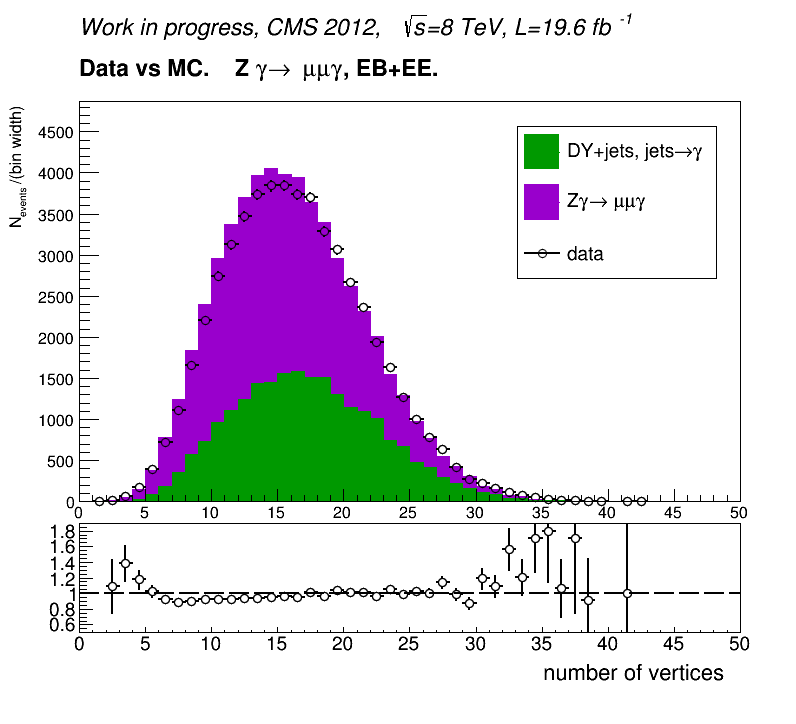
\includegraphics[width=0.45\textwidth]{../figs/figs_v11/MUON_ZGamma/PrepareYields/c_TotalDATAvsMC_EtaCommon__nVtx_noPU.png}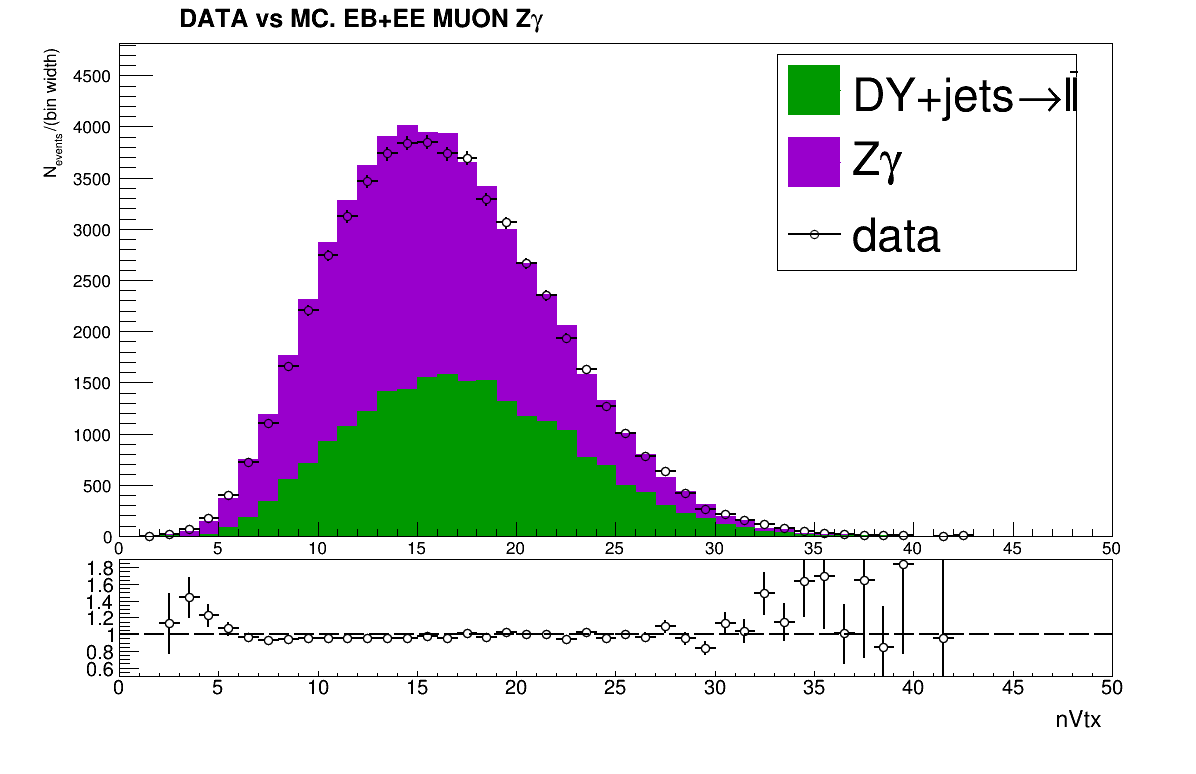
\includegraphics[width=0.45\textwidth]{../figs/figs_v11/MUON_ZGamma/PrepareYields/c_TotalDATAvsMC_EtaCommon__nVtx.png}
  \caption{Number of vertices of $Z\gamma$ candidates in the muon channel. Data vs MC. Left: no PU reweighting applied, right: PU reweighting applied. }
  \label{fig:DATAvsMC_nVtx}
  \end{center}
\end{figure}
